\chapter{Sharing Immutable Data}
\label{chapter:sharing-immutable-data}

If you examine any Java
heap, you will find that a
large amount of the data is duplicated. At one extreme, 
there are often thousands of copies of the same boxed
integers, especially 0 and 1. At the other extreme, there may be many
small data structures that have the same shape and data, and are never modified
once they are initialized. And, of course, duplicate strings are extremely common.
This chapter describes
techniques for sharing read-only data to avoid
duplication, including a few low-level mechanisms that Java provides.
\autoref{sec:literals} looks at sharing literal data, known at compile time. 
The rest of the chapter describes techniques for sharing more
dynamic data.

\section{Sharing Literals}
\label{sec:literals}

Duplicate strings are one of the
most common sources of memory waste, since even
small strings incur a large overhead. It is not uncommon to
see heaps with tens of thousands of copies of strings such as \code{"Y"} or
\code{"N"}. At 48 bytes a piece, these quickly add up.
Fortunately, it is not hard to eliminate string duplication.

One technique is to represent strings as  
literals whenever possible. Duplication problems arise because dynamically
 created strings
are stored in the heap without checking whether they already
exist. String literals, on the other hand, are stored in a
\emph{string constant pool} when classes
are loaded, where they are shared.

As an example, consider a document storage system that initializes each document
object before reading in metadata about that document.  A common
mistake is to create a new \code{String} from a \code{String} literal:

\begin{shortlisting}
	public Document() {
		name = new String("unknown");
		description = new String("unknown");
	}
\end{shortlisting}

Even though the standard library is smart enough to share the
underlying character array, 
this code will still create two new \code{String}
objects for every document. 
Compare that to the following:

\begin{shortlisting}
	public Document() {
		name = "unknown";
		description = "unknown";
	}
\end{shortlisting}

The \jre shares the \code{String} literal wherever it appears in
the code, even across classes. More important, in this example, is that now all
documents will share a single \code{String}. A similar, more maintainable
approach is to make the sharing explicit, by defining a \code{final
static} constant:

\begin{shortlisting}
	public class Document {
		public final static unknown = "unknown";
		..
		public Document() {
			name = unknown;
			author = unknown;
			..
		}
	}
\end{shortlisting}

A more dynamic version of the problem often occurs when data originates from 
an external source. Extending our example, suppose the
application reads in the metadata for each document as a set of property
name-value pairs. The code below builds each map directly from the
input. \code{getNextString()} returns a new
\class{String} for each property name and value.

\begin{shortlisting}
	public class DocumentProperties {
		protected Map<String, String> propertyMap;
		..
		
		public void handleNextEntry() {
			String propertyName = getNextString();  
			String propertyValue = getNextString();
			propertyMap.put(propertyName, propertyValue);
		}
	}
\end{shortlisting}

The \class{String}s stored in each map are created dynamically.
In applications of this kind, there is usually a lot of repetition of both
property names and values. If there are just a few distinct property names in all of the input pairs, these
property names will be duplicated many times in the heap.
However, if we know in advance what all of the property names are,
then we can define them once as \class{String} literals. For example:

\begin{shortlisting}
	public class DocumentProperties {
		// Property names
		final public static String format = "format";
		final public static String comments = "comments";
		final public static String timestamp = "timestamp";
		..
	}
\end{shortlisting}

When reading in the property names, we could check against these
literals, and share them as the keys in each map. 
Alternatively, a better stylistic choice would be to encode them as an
enumerated type. Like \class{String} literals, the \jre maintains a
single copy of each \code{enum} constant. Unlike \class{String}s,
you never have the option to allocate \code{enum} instances dynamically; they
are always shared constants. 

\begin{shortlisting}
	public class DocumentWithStaticProperties {
		public enum PropertyName = 
			{format, comments, creationDate, ... };
		..
		protected Map<PropertyMap, String> properties; 
		..
		void handleNextEntry() {
			PropertyName propertyName = 
				PropertyName.valueOf(PropertyName.class, getNextString()); 
			String propertyValue = getNextString(); 
			properties.put(propertyName, propertyValue); }
	}
\end{shortlisting}

The code reads in a property name, and returns a pointer to a shared \code{enum}
constant. \code{enum} types automatically provide for
efficient lookup by name, in addition to giving you type safety. In our
example, using an \code{enum} type would also allow us to save even more memory,
by switching from a \code{HashMap} to the smaller \code{EnumMap} to store each document's metadata.

Using literals to avoid duplication is only possible when values are known in advance.
\autoref{sec:sharing-pools} introduces the notion of a sharing pool for
sharing dynamic data. \autoref{sec:sharing-strings} describes
string interning, Java's built-in way to share strings.

\section{Sharing Pools}
\label{sec:sharing-pools}

Suppose an application generates a lot of duplicated data and the values
are unknown before execution. 
You can eliminate data duplication by using a \emph{sharing pool}, also known
as a \emph{canonicalizing map}. 
A sharing pool will eliminate not just duplicate data, 
but all of its associated overhead. Since many Java data structures employ 
delegation in their designs, sharing duplicate data can avoid
multiple levels of identical objects.

An example is shown in \autoref{fig:sharing-pool}. The example is from a
text processing system, which assigns a type to each word in a document.
Each type is identified by a \class{String} type name.
The complete set of word types is known only at run time, so an \code{enum}
type cannot be used.  In \autoref{fig:sharing-pool-a}, objects A and B
are words that have been classified as having the same type. 
\autoref{fig:sharing-pool-b} shows objects A and B sharing the type
structure, which is stored in a sharing pool. In this example, each use of a
shared structure saves three objects.

\begin{shortlisting}
public class WordInContext {
	private int  locationInDocument;
	private Type type;  // The word's role in the sentence
}

public class Type {
	final private String typeName;
}
\end{shortlisting}


\begin{figure}
\centering
	\subfigure[]{\label{fig:sharing-pool-a}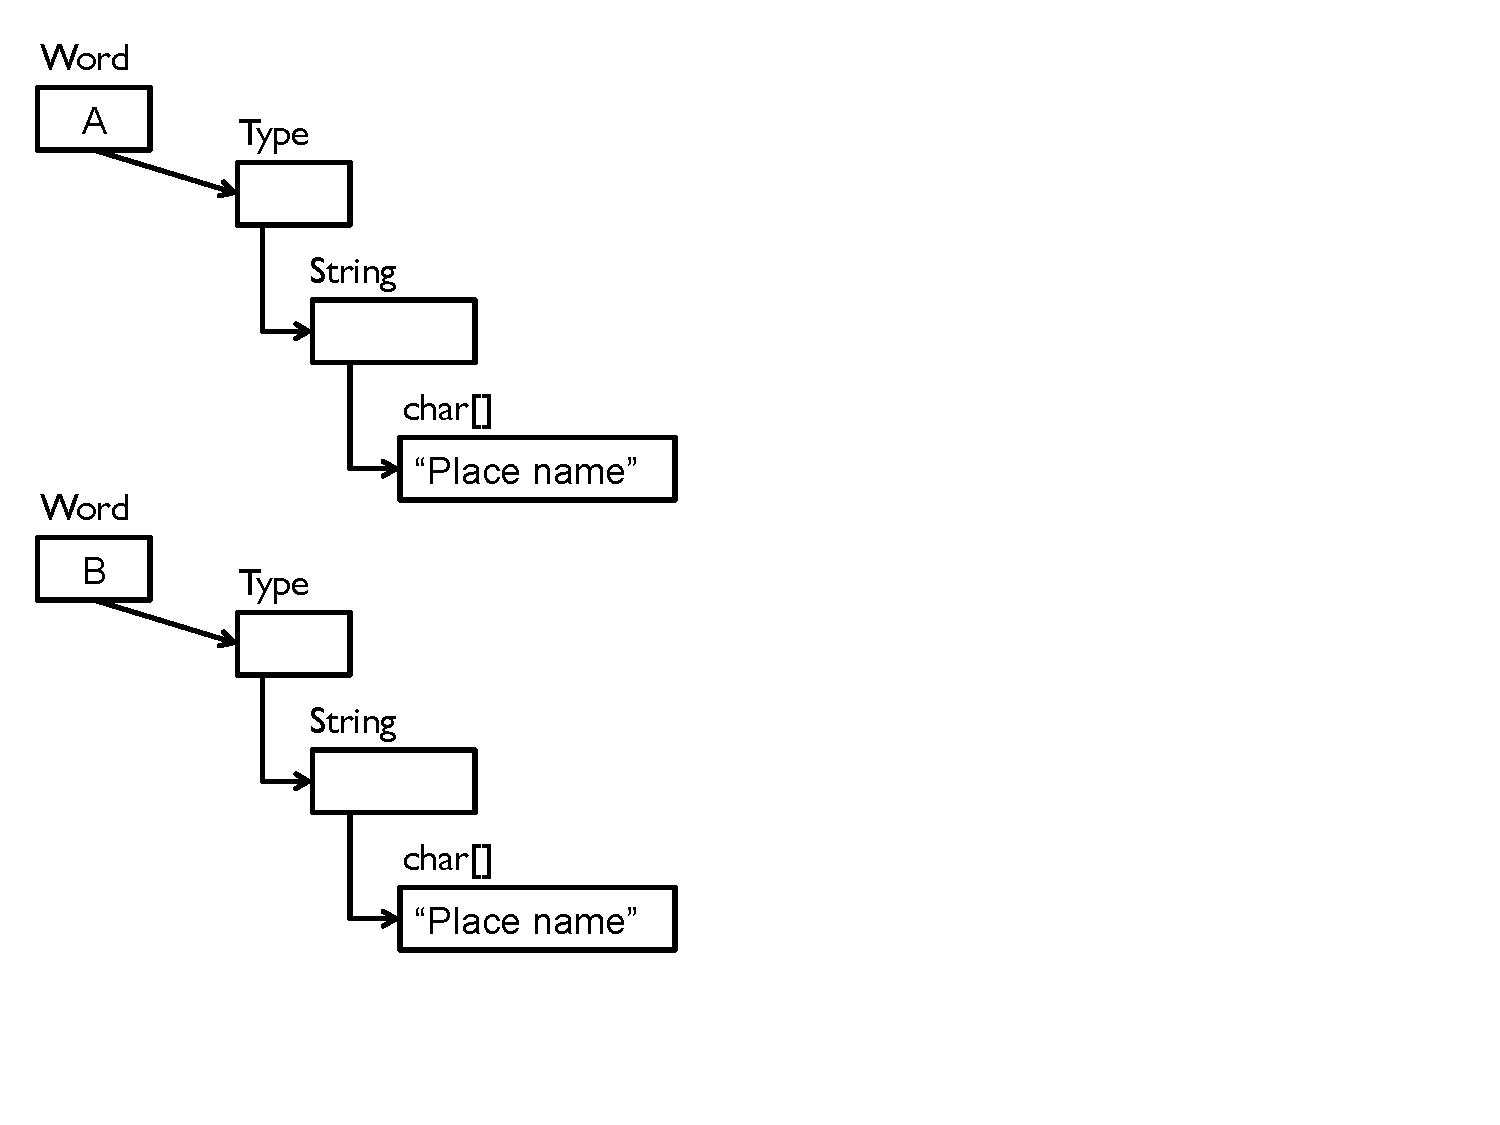
\includegraphics[width=0.3\textwidth]{part1/Figures/modelingdatatypes/sharing-pool-a.pdf}}
	\hspace{0.18\textwidth}
	\subfigure[]{\label{fig:sharing-pool-b}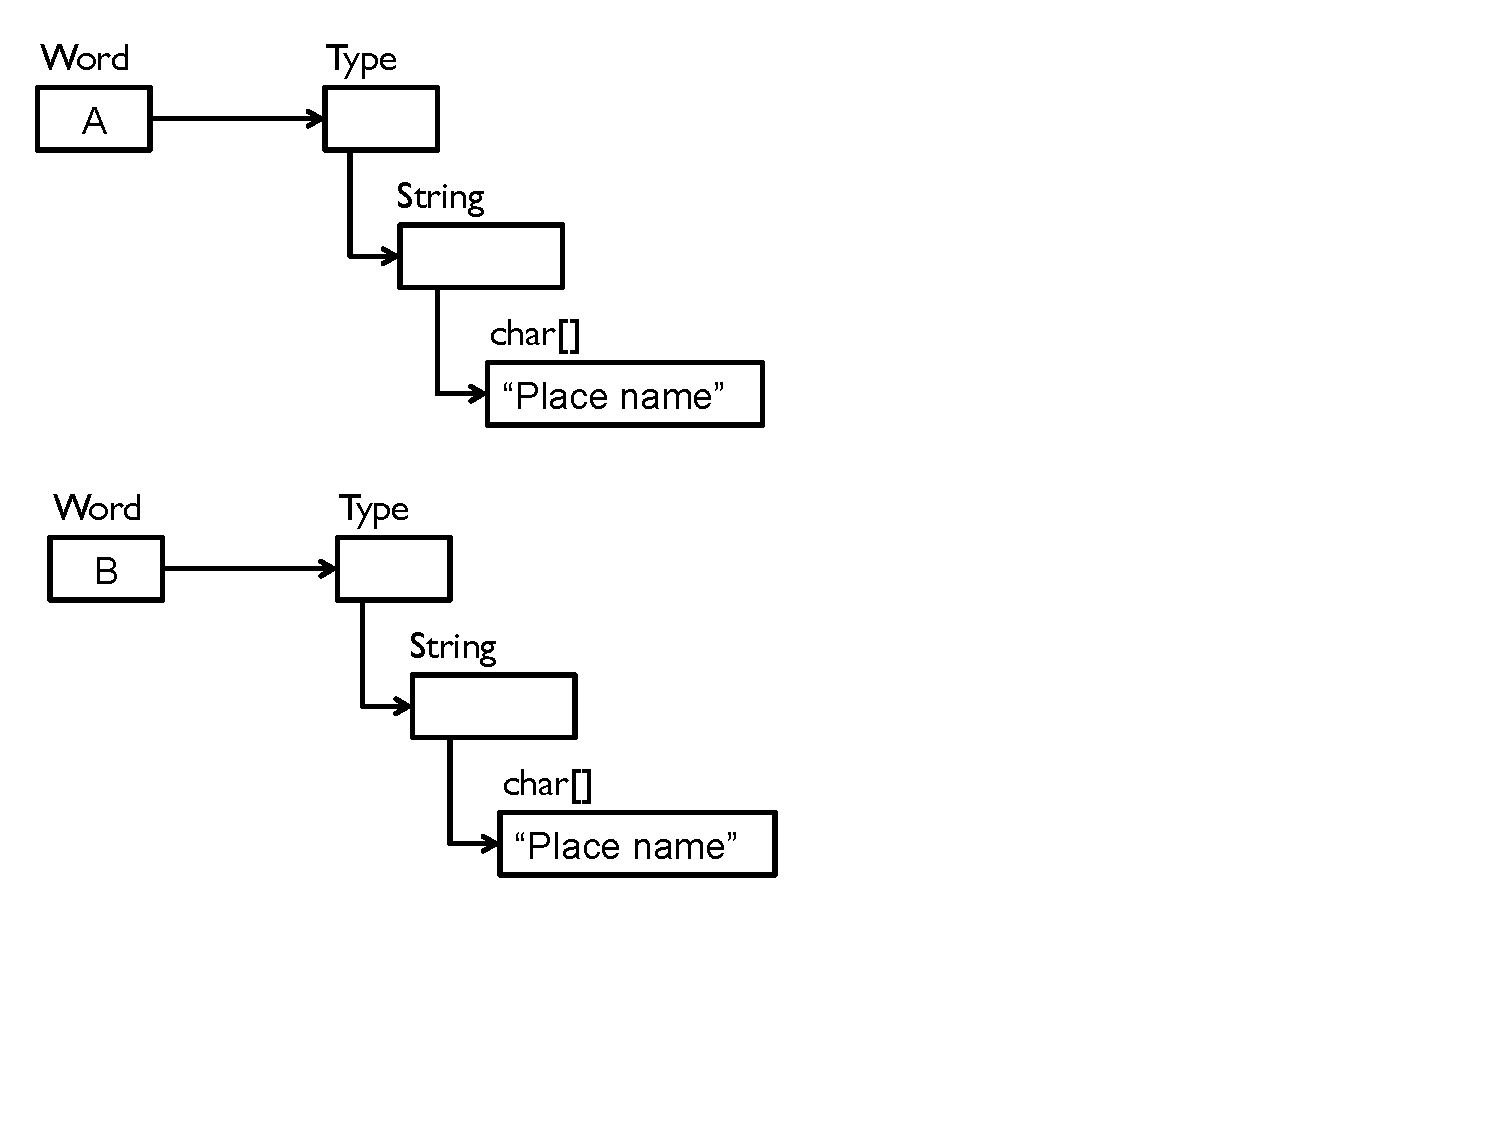
\includegraphics[width=0.445\textwidth]{part1/Figures/modelingdatatypes/sharing-pool-b.pdf}}
    \caption{(a) Words A and B point to duplicated data. (b) Words A and B
    share the same data, stored in a sharing pool.}
	\label{fig:sharing-pool}
\end{figure}

\callout{callout:sharing-pool}{Sharing Pool}{
A \emph{sharing pool} is a centralized structure
that stores canonical, read-only data that would otherwise be replicated in many
instances. A sharing pool itself is usually some sort of hash table, although it
could be implemented in other ways.
}

There are several issues that you need to be aware of before using a sharing
pool.
\paragraph{Shared objects must be immutable.} Changing shared data can
have unintended side effects. For example, 
changing the contents of the Type that A points to in
\autoref{fig:sharing-pool-b}, would also change the type of B.

\paragraph{The result of \code{equals} testing should be the same,
whether or not objects are shared.}
Always use \code{equals} to compare shared objects; never rely on \code{==}.
In \autoref{fig:sharing-pool},
\code{A.type == B.type} is false in \ref{fig:sharing-pool-a} and true in
\ref{fig:sharing-pool-b}, which can lead to very subtle bugs.
Some sharing pool implementations do not guarantee that all
duplicates will actually be shared. Avoiding \code{==} also allows
you to safely change your design, should you later decide to share a different set of instances, or to not share data at all.
\footnote{An argument sometimes heard for sharing data is that it will
allow for speedier comparisons, by letting the application use \code{==} rather
than \code{equals}. In fact, most
 \code{equals} methods already perform this optimization, with virtually
 identical performance to calling \code{==}
 directly.}
 
\paragraph{Sharing pools should not be used if there is limited sharing.}
A sharing pool itself can add
memory costs, typically the cost of a map entry for each instance stored in the
sharing pool.
If there is not much sharing, then the memory saved from
eliminating duplicates isn't enough to compensate for the
extra cost, and memory will be wasted instead of saved.  In \autoref{sec:quantifying-sharing-savings} is
a sample analysis of when it's worth sharing strings.

% NMM 20110614 i thought this was a good idea, but in Java, a reference will
% always be cheaper than an object, because of the header!
%\paragraph{The shared data items must be sufficiently large.} The size of the
%each pooled data item must be large, relative to the cost of a reference ---
%when using a pool, you still need to pay at least one reference cost for
%each use of the pooled items. 

\paragraph{Sharing pools can have performance costs.}
Sharing pools can sometimes add a performance cost when creating new instances
to be shared.  First, each new instance requires a lookup and possible
addition to the sharing pool. Second, in a multithreaded
environment, checking and adding to the sharing pool can introduce latency if the sharing pool is synchronized.
The use of shared instances, however, does not incur any extra
time costs.

\paragraph{Sharing pools should be either stable or garbage collected.} 
In Figure~\ref{fig:sharing-pool-b}, the sharing pool stores an object
that no other object is pointing to. Over time, a sharing pool can fill up with
garbage, that is, items that were once needed but not any more. If the
sharing pool is not purged of these unused items, there will be a leak, 
eventually using up more and more memory. However, if there are only a small
number of shared instances, or if the set of shared instances is unchanging for the lifetime of the pool,
then garbage collection need not be a concern.

Fortunately, Java provides a few built-in mechanisms that take care of
these concerns for some common cases.

\section{Sharing Strings}
\label{sec:sharing-strings}
\index{Interning}

%Before storing a 
%To use a sharing pool, before storing a new
%\class{String}, first check the pool to see if it is already there. If it is,
%reuse it; otherwise, add the new string to the pool. 
%One catch is that if you end up adding many strings to
%the pool that are never reused, then you will waste memory, since the pool
%structure itself has overhead. So you need to have a good idea
%which strings are likely to have duplicate values.

Since \class{String} duplication is so common, Java provides a built-in
pool for sharing \class{Strings}. To share a new
\class{String}, you simply call the method \code{intern} on it, and 
everything is taken care of automatically. Both the \class{String}
object and its underlying character array are shared. Since
\class{Strings} are immutable, sharing is safe.
However, the rule about not using \code{==} still holds on shared
\class{Strings}.  Remember that only some
\class{Strings} will be shared in any application, namely those specific
instances that you choose to intern.

In the example from ~\autoref{sec:literals},
\class{DocumentWithStaticProperties} eliminates property
name duplication, but only if all the property names are known in advance.
Suppose you know there are not many distinct property names overall, but you
don't know what they are in advance. In this case, property names
are perfect candidates for \class{String} interning.
\begin{shortlisting}
 
 class DocumentWithInternedProperties {
    void handleNextEntry() {
       String propertyName = getNextString().intern(); 
       String propertyValue = getNextString();
       propertyMap.put(propertyName, propertyValue);
    }
}
\end{shortlisting}

The call to \code{intern} adds the new property name \class{String}
to the internal string
pool if it isn't there already, and returns a pointer to it. Otherwise, the
new \class{String} is a duplicate, and a previously saved \class{String} is
returned instead. 

There is a memory overhead cost for each shared
\class{String}, so interning \class{Strings} indiscriminately will waste memory.
In this example, there is probably a lot of duplication
among the property values too. However, we might only want to
add interning for those properties with the most duplication. For example, a property
for the document format would have just a few distinct values, and is a good
candidate for interning.
On the other hand, a timestamp property would be a poor candidate. In this way
we would get the maximum benefit from sharing, while keeping the overhead to a
minimum. 

The \jre maintains a map in native memory to keep track of the interned
\class{String}s.
The interned \class{Strings} themselves are stored in a separate heap known as
the \emph{perm space}. 
Exceeding the size of the perm space will result in an exception:
\code{java.lang.OutOfMemoryError:PermGen space}
\footnote{This is an issue only for the \oracle \jre. The \ibm \jre places no 
fixed limit on interned \code{Strings}.}.
There are parameters to adjust the perm space size. See \autoref{chapter:jre-options} for details. 
Fortunately, the \jre performs garbage collection on the
internal string pool, so there is no danger of a memory leak.
\index{Permspace Heap}

The built-in interning mechanism is synchronized, and can incur a latency cost
in a multithreaded environment, when new \class{Strings} are interned.
The book Effective Java\cite{EffectiveJavaBook}, pp. xxx-yyy, gives an example
of how to build a concurrent sharing mechanism for \class{Strings}.

 %    * Literal strings within the same class in the same package represent
%     references to the same String object. * Literal strings within different
 %    classes in the same package represent references to the same String
%     object. * Literal strings within different classes in different packages
 %    likewise represent references to the same String object. * Strings
 %    computed by constant expressions are computed at compile time and then
   %  treated as if they were literals. * Strings computed by concatenation at
    % run time are newly created and therefore distinct.
\section{Sharing \class{Integers} and Other Boxed Scalars}

As of \javafive, the Java library provides sharing pools for
\class{Integers} and some of the other boxed scalars. These pools
work differently from \class{String} interning, where you must always create a
new \class{String} first and then call its \code{intern} method. To take
advantage of the \class{Integer} pool, simply call the factory method
\code{Integer.valueOf(int i)} whenever you need a new \code{Integer}.
The \class{Integer} pool is initialized with all the \class{Integers} in a fixed
range, from -128 to 127 by default. The factory method returns a
pointer to an \class{Integer} in the pool, provided \code{i} is in
range; otherwise it returns a new \class{Integer}. 
The idea is  that the most commonly
used integers (at least in many applications) will be shared. There is a
parameter to change the upper limit of the range -- see
\autoref{chapter:jre-options} for details. Note that
behind the scenes, Java's autoboxing feature uses these same pools
to share some of the instances it creates.

%For example,
%the code in \autoref{fig:integer-sharing-pool} stores \class{Integers} from 1
% to 500 in an array.
%\code{valueOf} returns an existing \class{Integer}
%for the first 127 numbers, and, for the rest of the numbers, \code{valueOf}
%returns a new \class{Integer} instance.  

%\begin{wrapfigure}{r}{0.4\textwidth}
%\centering
%\begin{framedlisting}
%for (int i=1; i<=500; i++) {
% numbers[i] = Integer.valueOf(i);
%}
%\end{framedlisting}
%\caption{By using the \code{valueOf} method, you can leverage the standard
%library's integer sharing pool.}
%\label{fig:integer-sharing-pool}
%\end{wrapfigure}

Because the \class{Integer} sharing pool is pre-initialized and fixed in size,
it's always a good idea to call \code{Integer.valueOf}, instead of
the constructor, whenever you need a new \class{Integer}. The pooling aspect is
very cheap, and you never have to worry about garbage collection, wasting memory, or concurrency issues.
You do have to be careful, however, to avoid using \code{==} to compare
\class{Integers}, since only some instances are actually shared. 
As always, using \code{equals} is a better practice.

The Java library provides a \code{valueOf} method for each of the boxed
scalars. \code{Character} and \code{Short} pools work in a similar fashion
to \code{Integer}, sharing only values within a range. For some types,
such as \class{Float}, there is no sharing actually implemented. For
\class{Boolean} and \class{Byte}, a shared constant is returned for every possible value. 
In general, there is no penalty for always using \code{valueOf}.

The exception to this rule is if you expect to have many copies
of values outside the range of what the built-in pool
actually shares. In this case you will not get the benefit of the built-in
mechanism, and it may be worth implementing your own sharing instead.  When
sharing something as small as a boxed scalar, however, there must be a very
high degree of duplication to make up for the overhead of your
sharing mechanism.

\section{Sharing Your Own Structures}
\label{sec:canonicalizing-maps}

Beyond strings and boxed scalars, there can be other kinds of
duplicated data structures that consume large portions of the heap. 
There is no built-in Java mechanism to share data
in general, so you have to implement a sharing pool from
scratch. All of the sharing pool issues from \autoref{sec:sharing-pools} need
to be addressed. The shared structures must be immutable, they must not be
compared using \code{==}, there must be sufficient memory savings from sharing
to justify the sharing pool, and the sharing pool must not cause a memory leak. 

There are two common styles of implementing your own sharing pool, depending on
the complexity of the data being shared.  We illustrate both in this section. 
For the purposes of this discussion we assume that the set of shared data is
always needed throughout the run, so there is no need to worry about garbage collection. In
\autoref{sec:sharing-pools-safety} we revisit these two examples, and show how
to implement sharing pools with garbage collection.  
We leave the addition of concurrent access as an exercise. 

\paragraph{Sharing simple data.} To illustrate one common style of
user-written sharing pool, consider a graph where every node has an
annotation, and many of these annotations are duplicates.
Each annotation is a single, immutable 
object, containing just a few scalar fields. The graph is modified
dynamically, and a new annotation may be assigned to a node at any
time. Assume for now that the same universe of annotations is needed for the
duration of the run.
The main requirement is the ability to find and
retrieve existing annotations quickly to share them.

\begin{wrapfigure}{r}{0.5\textwidth}
\centering
\begin{framedlisting}
HashMap<Annotation, Annotation> canonicalizingMap;
\end{framedlisting}
\end{wrapfigure}

Interestingly, none of the common collection classes meet this requirement
out of the box. A \class{HashSet} can store \class{Annotation}s uniquely, but
retrieving an existing \class{Annotation} is not easy. The \class{HashSet}
can let you know whether an equivalent item already
exists in the set, but can not return that item quickly. To get the
preexisting item, you would need to iterate over the entire set. The
most common approach is to use a
\class{HashMap} that maps the \class{Annotation} to itself, as shown on the
right. This design assumes that an \class{Annotation} can serve as its own key.
In other words, that the \code{hashcode} and \code{equals} methods are
defined on \class{Annotation} so that they ensure uniqueness. Note that, unless overridden, \code{equals} is
implemented as \code{==}, so sharing data structures typically requires writing
a new \code{equals} method.  

Callers must create an instance of \class{Annotation} in order
to find out whether it's already in the shared pool. This
is similar to the pattern of using \code{String.intern}, where you create a new
\code{String} in order to see if a matching shared \code{String} exists. Therefore, this type
of canonicalizing map only makes sense when sharing relatively simple data
that is inexpensive to create.

\begin{wrapfigure}{r}{0.5\textwidth}
\centering
\begin{framedlisting}
HashMap<String, Type> canonicalizingMap;
\end{framedlisting}
\end{wrapfigure}

\paragraph{Sharing more complex data.} Suppose that we would like to
share more complex data, such as the type information from \autoref{fig:sharing-pool}. In this example, the type is
uniquely identified by a \class{String} type name. Each shared structure
consists of three objects. Rather than asking the programmer to create a new \class{Type} structure only to discover
that it exists in the pool, we can instead use the type name as the key, as
shown on the right. That way callers of the sharing pool only have to create a
\code{String} in order to find or retrieve the \class{Type}. In this example we save the creation of
one object for each new instance of the structure created.  For more complex
structures the savings can be much greater.

\paragraph{} Whichever of these two approaches you use, it's a good idea to hide
the use of the sharing pool behind a factory method. That will make it easier to make
changes later, should you find that sharing is not worthwhile.

%A common term for this structure is a \emph{canonicalizing map}.

\index{Canonicalizing Map}

\section{Quantifying the Savings}
\label{sec:quantifying-sharing-savings}

Before implementing a sharing scheme, we can estimate the
space savings to make sure it's worth
the effort, and to make sure it doesn't cause a net gain in
memory usage. Here is a sample analysis of sharing \class{String}s.
This style of analysis can be applied to other types of shared data.

First, we'll need to estimate
a few properties of the data we are considering sharing. For this example,
we'll start with a set of one million \class{String}s, and make the
simplifying assumption that they are all the same size, ten characters each.
Without any sharing, this data would require 64 bytes per \class{String},
or 64 Mbytes in total. Next, we'll need the overhead
of the sharing mechanism, in this case Java's built-in string interning. The
\jre stores its map of shared strings in native memory. We'll assume that the
native map costs 20 bytes on average for each distinct value\footnote{This is
an approximation, for illustration purposes, of what
a native weak hash map might cost on a 32-byte \jre.}. 

Finally, we'll look at the degree of duplication in the data set. One
useful measure is the ratio of distinct values to the total number of items in the set. 
A lower fraction, closer to 0, means there are more duplicates, since
there are fewer distinct values in the set. A higher value, closer to 1, means
there are more distinct values, so less duplication. 

\begin{figure}
\centering
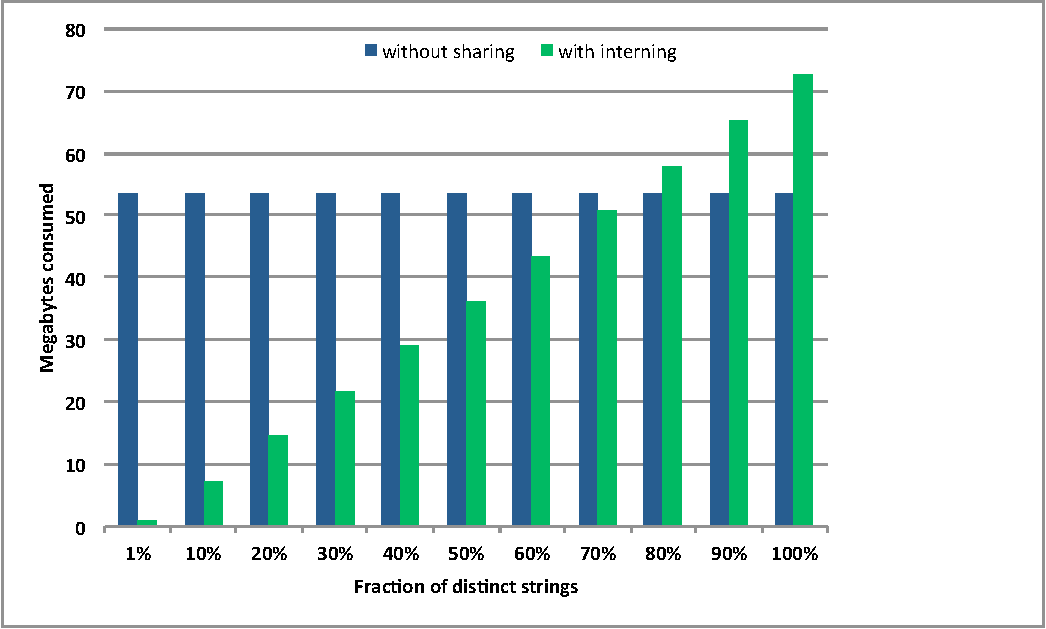
\includegraphics[width=\textwidth]{part1/Figures/modelingdatatypes/sharingpool_consumptionchart.pdf}
	\caption{Comparing the memory consumed by
	one million ten-character \class{String}s, stored individually vs. with
	interning.
	The chart shows how the savings (or waste) varies with the degree of
	distinctness of the data. 10\%
	means there are only 100,000 distinct strings.}
	\label{fig:sharing-savings}
\end{figure}

\autoref{fig:sharing-savings} shows how the cost of sharing strings
varies based on this ratio. Each data point compares not sharing
(the left bar) against
interning (the right bar). There is considerable savings with even
a moderate amount of duplication. For example, when distinct values
are 50\% of the total number of \class{String}s, so on average 2 identical \class{String}s per value, 22
Mbytes are saved. When the
percent is above 76\%, however, memory is wasted, since there isn't enough duplication to justify the extra overhead.

\callout{callout:sharing-savings}{Estimating the Savings from Sharing}{
\index{Sharing Savings Calculation}
Let:
\begin{eqnarray} 
N &=& the\ number\ of\ items\ in\ the\ data\ set  \nonumber \\
S &=& the\ average\ size\ in\ bytes\ of\ a\ data\ item \nonumber \\
D &=& the\ ratio\ of\ distinct\ values\ to\ total\ number\ of\ items \nonumber
\\
E &=& the\ average\ per\ entry\ overhead\ of\ the\ sharing\ mechanism \nonumber
\end{eqnarray}

In a shared implementation, a fraction D of the total items incur the
overhead of the sharing pool. The savings is the cost difference between
the non-shared and shared versions:

\begin{eqnarray}
N \cdot S\ \ -\ N \cdot D \cdot (S+E) \nonumber
\end{eqnarray}

The savings will be positive whenever:
\begin{eqnarray}
D &<& \frac{S}{S+E} \nonumber
\end{eqnarray}

} 

The callout shows a general formula for approximating the savings of sharing any
kind of data.  
%In real applications, of course, there's usually more variation
%in the data items than in our simplified example, so we look at the
%average size of the data. 
If you use a standard Java
\class{Map} class as your sharing mechanism, the overhead will typically be
higher than the overhead of \class{String} interning.
Therefore, your data must have either more duplicates or
larger duplicate items, compared to our example, in order to achieve comparable
savings. If the map needs to provide for garbage collection, the overhead will
be higher still.
See \autoref{sec:large-collections}
for estimating the per-entry cost of a map.

\section{Summary} 
Many Java heaps are filled not only with high-overhead data structures, but
with many identical copies of them. Sharing read-only
data can provide big memory savings with little downside. There are many
techniques available:

\begin{itemize}
  \item To share a small number of values that are known at compile time, use
  \class{String} literals, \code{enum} constants or \code{final static}s.
  \item The \jre maintains a sharing
  pool for \class{Strings}. Use \class{String} interning to make use of this
  sharing pool.
  \item The standard library maintains fixed-size pools for
   a range of \class{Integers} and some of the other boxed scalars. You
   can take advantage of these by using \code{valueOf} factory methods, instead
   of constructors, to create boxed scalars.
   \item You can implement a sharing pool for your own datatypes using
   \class{Map} classes. To keep down the cost of creating new instances, choose
   the right pattern for the data: \code{Map<value, value>} for
   simple data, and \code{Map<key, value>} for sharing larger structures.
\end{itemize}

When sharing data, remember these four rules:
\begin{itemize}
  \item Shared structures must be immutable.
  \item The result of \code{equals} testing should be the same, whether or
not objects are shared. In application code, use \code{equals} rather than
\code{==} to test for equality.
  \item Sharing pools should not be used if there is limited sharing, and the
  overhead of the pool will outweigh the benefit.
  \item The pool must provide for garbage collection of shared objects
  that are no longer needed, unless: 1. the set of shared objects is
  small, or 2. the set of shared objects is stable for the lifetime of the
  pool.
\end{itemize}

The techniques described in this chapter for sharing immutable
data can lead to substantial savings for many applications.  All of these
techniques are within the bounds of standard, object-oriented programming
practice. Later in the book, in \autoref{chapter:large-long-lived}, we look at
bulk storage and sharing techniques that stretch beyond the normal Java box in
order to achieve even greater space savings. 






